%\noindent 

%%% obvious!
%Today's popular online services, such as web search, video streaming,
%and social networks, are all powered by large data centers. In
%addition to these public services, a lot of scientific research and
%business activities are migrating onto cloud
%computing\cite{Ferdman:2012:CCS:2150976.2150982,mrbs}. Table \ref{tbl:apps}
%lists several popular classes of applications that are running on the
%cloud.
%
%
%
%\begin{table}[!h]
%	\caption{Typical cloud computing applications.}
%	\centering
%		\begin{tabularx}{\columnwidth}{|l|X|}
%			\hline
%			Class                          & Examples                         \\
%			\hline
%			Data analytics   & bioinformatics\\ 
%			& business intelligence\\
%			\hline
%			Graph analytics  & social networks\\ 
%			& recommendation \\
%			\hline
%			Web search       & text processing\\
%			& recommendation\\
%			\hline
%			\end{tabularx}
%	\label{tbl:apps}
%\end{table}
%
%Two main characteristics of the above applications are large dataload
%and high parallelism. In 2008, Google processed 20 PB of data with
%MapReduce each day; in April 2009, a blog revealed eBay's 2 enormous
%data warehouses: one with 2 PB of data and the other with 6.5 PB of
%data; shortly thereafter, Facebook also shocked the world with its 2.5
%PT of user data which kept growing at 15 TB per
%day \cite{lin2010data}. Without high parallelism, these huge amount of
%data are beyond our capability of processing. 

%If a task is delayed 
%We consider a cloud computing environment to be a distributed job
%which is made up of a series of tasks executing a job
%which is composed of multiple tasks, each of size W , executing in
%parallel on different com- puting nodes, as depicted in Figure 2. For
%the job to complete, all tasks must finish. If a task is de- layed
%then all tasks must wait for the completion of the slowest task for
%the job to complete.
%
%For each job that processes these data, there are usually multiple
%phases that execute in sequence. During each phase, workload is
%splited into tasks and processed in parallel to speed up the whole
%process. A job of 2 phases is illustrated in
%Figure \ref{fig:system_model}.


%\section{CC Workload Characterization}

Cloud computing workload ranges from business applications and
intelligence, to analytics and social networks mining and log
analysis, to scientific applications in various fields of sciences and
discovery. These applications exhibit different behaviors, in term of
computation requirements and data access patterns. While some
applications are compute-intensive, others involve the processing of
increasingly large amounts of data. The scope and scale of these
applications are such that an instance of a job running one of these
applications requires the sequential execution of multiple computing
phases; each phase consists of thousands, if not millions, of tasks
scheduled to execute in parallel and involves the processing of a very
large amount of data~\cite{lin2010data,Ferdman:2012:CCS:2150976.2150982}. This
model is directly reflective of the \emph{MapReduce} computational
model, which is predominately used in
Cloud Computing \cite{mrbs}.  An instance of this model, is depicted in Figure \ref{fig:system_model}.


\begin{figure}[!h]
	\begin{center}
		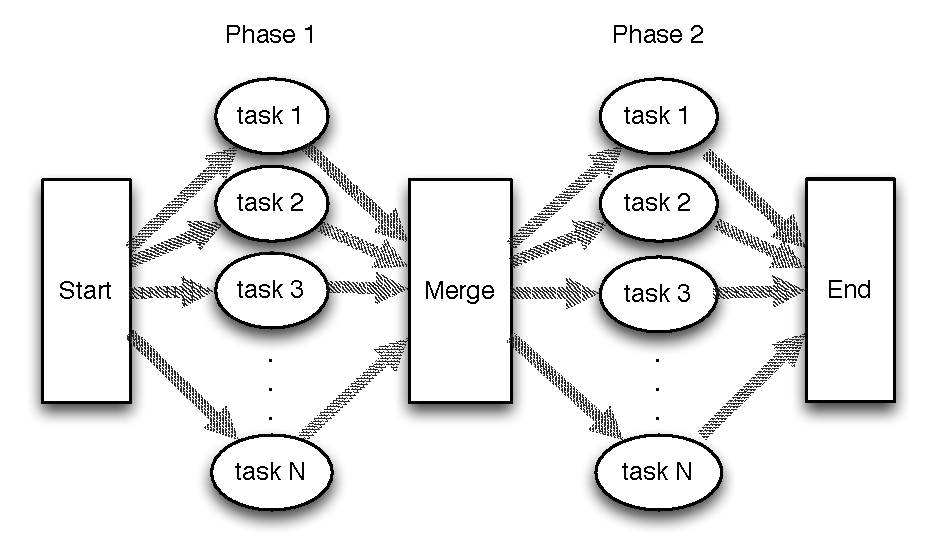
\includegraphics[width=\columnwidth]{diagrams/system_model_1.pdf}
	\end{center}
	\caption{Cloud computing execution model with 2 phases.}
	\label{fig:system_model}
\end{figure}

Each job has a targeted response time defined
by the terms of the SLA. Further, the SLA defines the amount to be
paid for completing the job by the targeted response time as well as
the penalty to be incurred if the targeted response time is not
met. 

Each task is mapped to one compute core and executes at a speed, $\sigma$. The partition of the job among tasks is
such that each task processes a similar
workload, $W$. Consequently, baring failures, tasks are expected to
complete at about the same time. Therefore, the minimal response time
of each task, when no failure occurs, is
$t_{min}~=~\frac{W}{\sigma_{max}}$, where $\sigma_{max}$ is the maximum speed. This is also the minimal response
time of the entire phase. 

As the number of tasks increases, however, the likelihood of a task
failure during an execution of a given phase increases
accordingly. This underscores the importance of an energy-efficient
fault-tolerance model to mitigate the impact of a failing task on the
overall delay of the execution phase. The following section describes
Shadow Replication, a fault-tolerant, energy-aware computational model to achieve profit-maximizing,
energy-efficient resiliency in cloud computing.


%\noindent
%We consider a job running in a cloud computing environment to be
%comprised upon multiple phases that execute in sequence. A two-phase
%job is depicted in Figure \ref{fig:system_model}. During each phase
%multiple tasks are executing in parallel. Each task contains the same
%amount of workload, denoted as $W$. If a task is delayed then all
%tasks must wait for the completion of the slowest task for that phase
%for the job to complete. This model is directly reflective of the
%map-reduce execution model used predominately in cloud computing.
%
%The large amount of data being
%processed~\cite{lin2010data,Ferdman:2012:CCS:2150976.2150982} requires
%the use of thousands, if not millions, of tasks during each phase. As
%the number tasks increases, the likelihood of failure during an
%individual phase will also increase. Fault tolerance is critical at
%the phase-level because the delay of one task results in a delay of
%the entire phase. Hence, techniques such as shadow replication would
%be applied to each phase independently. Due to this independence
%between phases, we consider a single phase job during our analysis.
%
%%For the job to complete, all tasks must finish its workload of
%%$W$. If a task is delayed then all tasks must wait for the completion
%%of the slowest task for the job to complete.
%
%We assume that each executing task is mapped to one computing core and
%executes at a maximum speed of $\sigma_{max}$. Therefore, the minimal
%response time of each task, when no failure occurs, is
%$t_{min}=\frac{W}{\sigma_{max}}$, which is also the minimal response
%time of the entire job.
%
%Each job has a targeted response time defined by the terms of the
%SLA. Further, the SLA defines the amount to be paid for completing the
%job by the targeted response time as well as the penalty to be
%incurred if the targeted response time is not met. We will discuss
%this in detail in Section~\ref{sla_reward_model}.
%
%
%%In the following section, we assume the above job execution model and
%%describe a profit-based optimization framework to compute the optimal
%%speeds of shadow replication. In this framework, it is assumed that
%%failures can be detected.  While this is the case in many computing
%%environments, there are cases where failure detection may not be
%%possible. To address this limitation, we propose a sub-optimal shadow
%%replication scheme, whereby both the main process and the shadow
%%execute independently at stretched speeds to meet the expected
%%response time, without the need for the main processes failure
%%detection.
